\chapter{Related Work} \label{Related Work:Radio Astronomy}
%Summary: 2 major sections, 1 about past radio instrumentation, 1 about automatic mapping\\
%Goal: Explain why we can mesh them together successfully in this case\\
%State: Can be written now \\
%List of references already compiled into Papers archive \\

%TODO: Intro
\section{Radio Astronomy} \label{Related Work:Radio Astronomy}
%\subsection{Digital Signal Processing for Radio Astronomy}
The need for high bandwidth processing manifests in many different radio astronomy applications.
Keeping up with increasing computation demands has often resulted in the specialized design of spectrometers.

%TODO: Intro
\subsection{Distributed FX Correlator (DiFX)}

%DiFX (Distributed FX Correlator) is a scalable software implementation
The DiFX Correlator is a scalable software implementation of an FX Correlator  \cite{Deller:2007wy}.
DiFX was designed as a software correlator that targets CPUs in order to maintain flexibility in the design.
The DiFX correlator was originally developed to do VLBI (Very Long Baseline interfereometery). 

%TODO: If you have a cluster available�
%Why do cpu-only?
%It�s easy
%Compared to 27 antenna 2GHz EVLA in New Mexico

 
%Describe the VLA


%TODO: expand on VLBI
%TODO: doesn't need to be real time (using recorded data)

%Designed for VLBI (Very Long Baseline Interferometry)



\begin{figure}[h!]
  \centering
    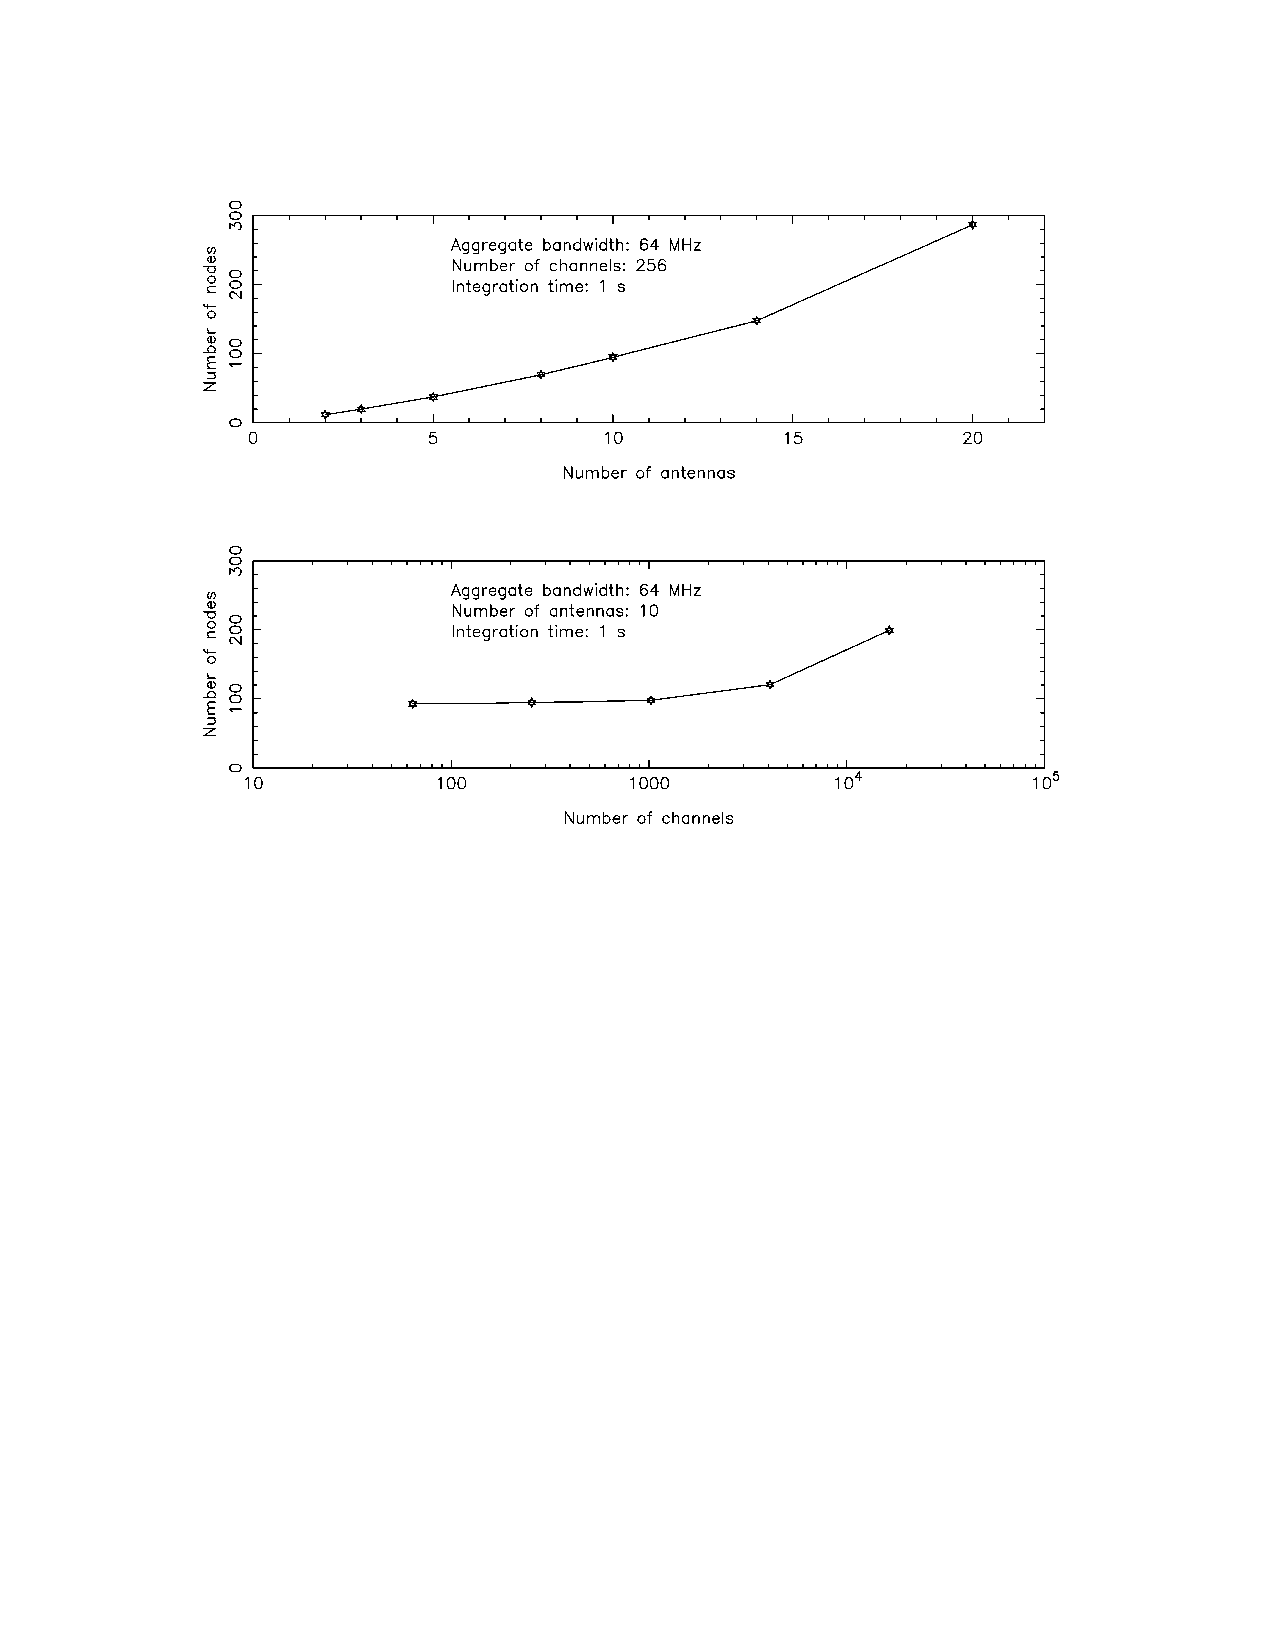
\includegraphics[width=\textwidth]{Images/C3/difx_scaling.pdf}
  \caption[DiFX Correlator Benchmarks]{DiFX Correlator Benchmarks (reprinted from \citeauthor{Deller:2007wy} \cite{Deller:2007wy})}
  \label{fig: C3/difx_scaling.pdf}
\end{figure}

Unfortunately, the flexibility of the software implementation comes at a high cost.
Figure \ref{fig: C3/difx_scaling.pdf} shows the resources required
Nearly 100 nodes are required to cross correlate 64 MHz of bandwidth from 10 antennas. 

\subsection{LOFAR}
\begin{figure}[ht!]
  \centering
    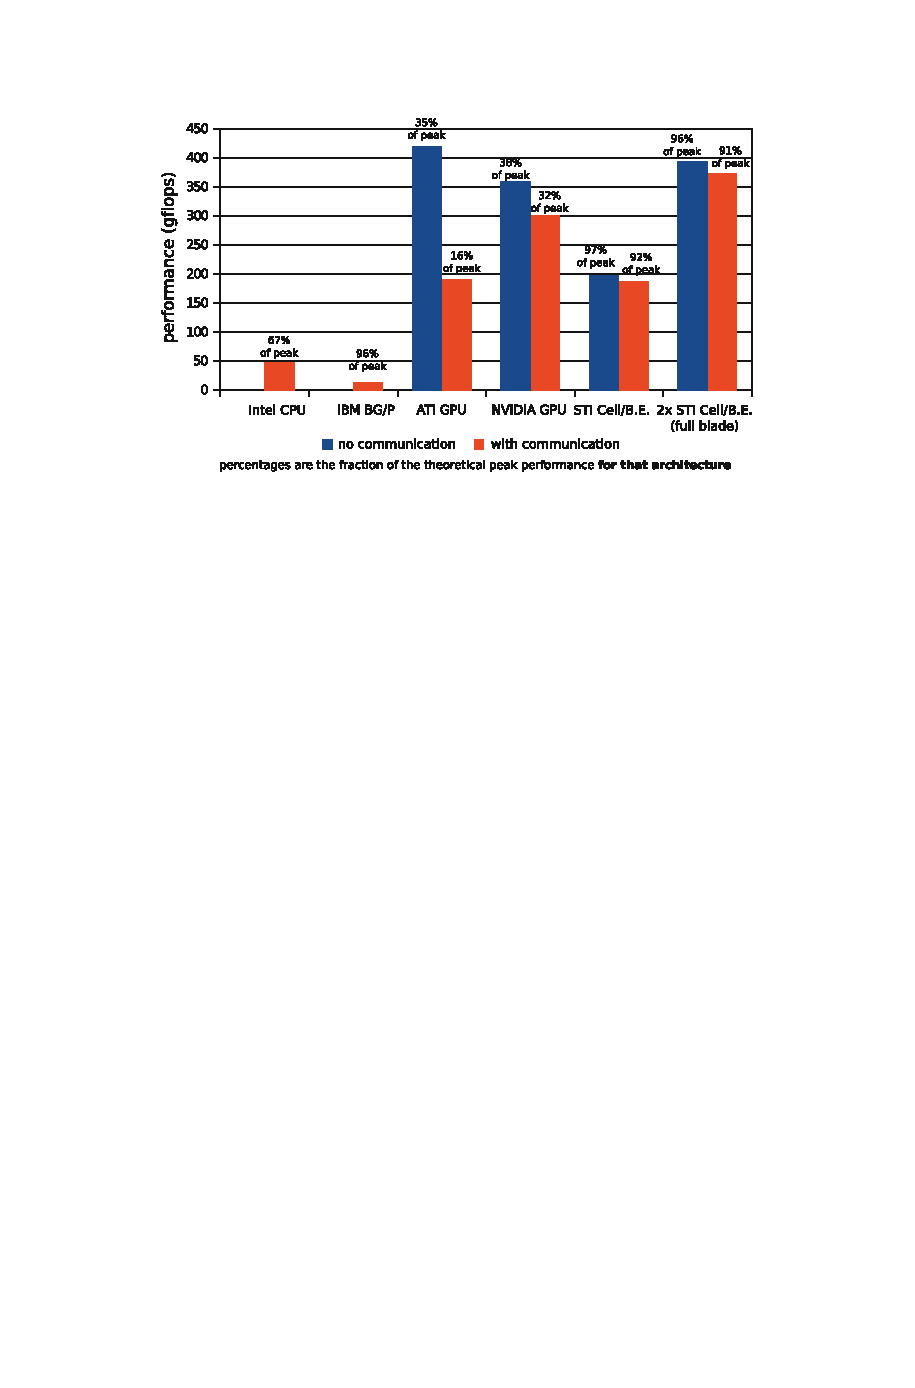
\includegraphics[width=\textwidth]{Images/C3/lofar_performance.pdf}
  \caption[LOFAR Correlator Performance]{LOFAR Correlator Performance (reprinted from \citeauthor{vanNieuwpoort:2009p1253} \cite{vanNieuwpoort:2009p1253})}
  \label{fig: C3/lofar_performance.pdf}
\end{figure}
%On a blue gene, real time but still costly power hungry solution 64 stations
%TODO: read this paper
Like DiFX, the correlator for Low-Frequency Array for Radio Astronomy (or LOFAR) was also built using CPUs \cite{vanNieuwpoort:2009p1253}.
This project used a Blue Gene BG/P %TODO: check this
to implement a 64 station correlator.
The implementation got very high performance out of the cluster, 96\% of the peak, but required an entire cluster and required finely tuned code to achieve that performance. 


\subsection{xGPU}
xGPU is a CUDA package that implements the cross-correlation
%TODO: add another graph from paper
\begin{figure}[ht!]
  \centering
    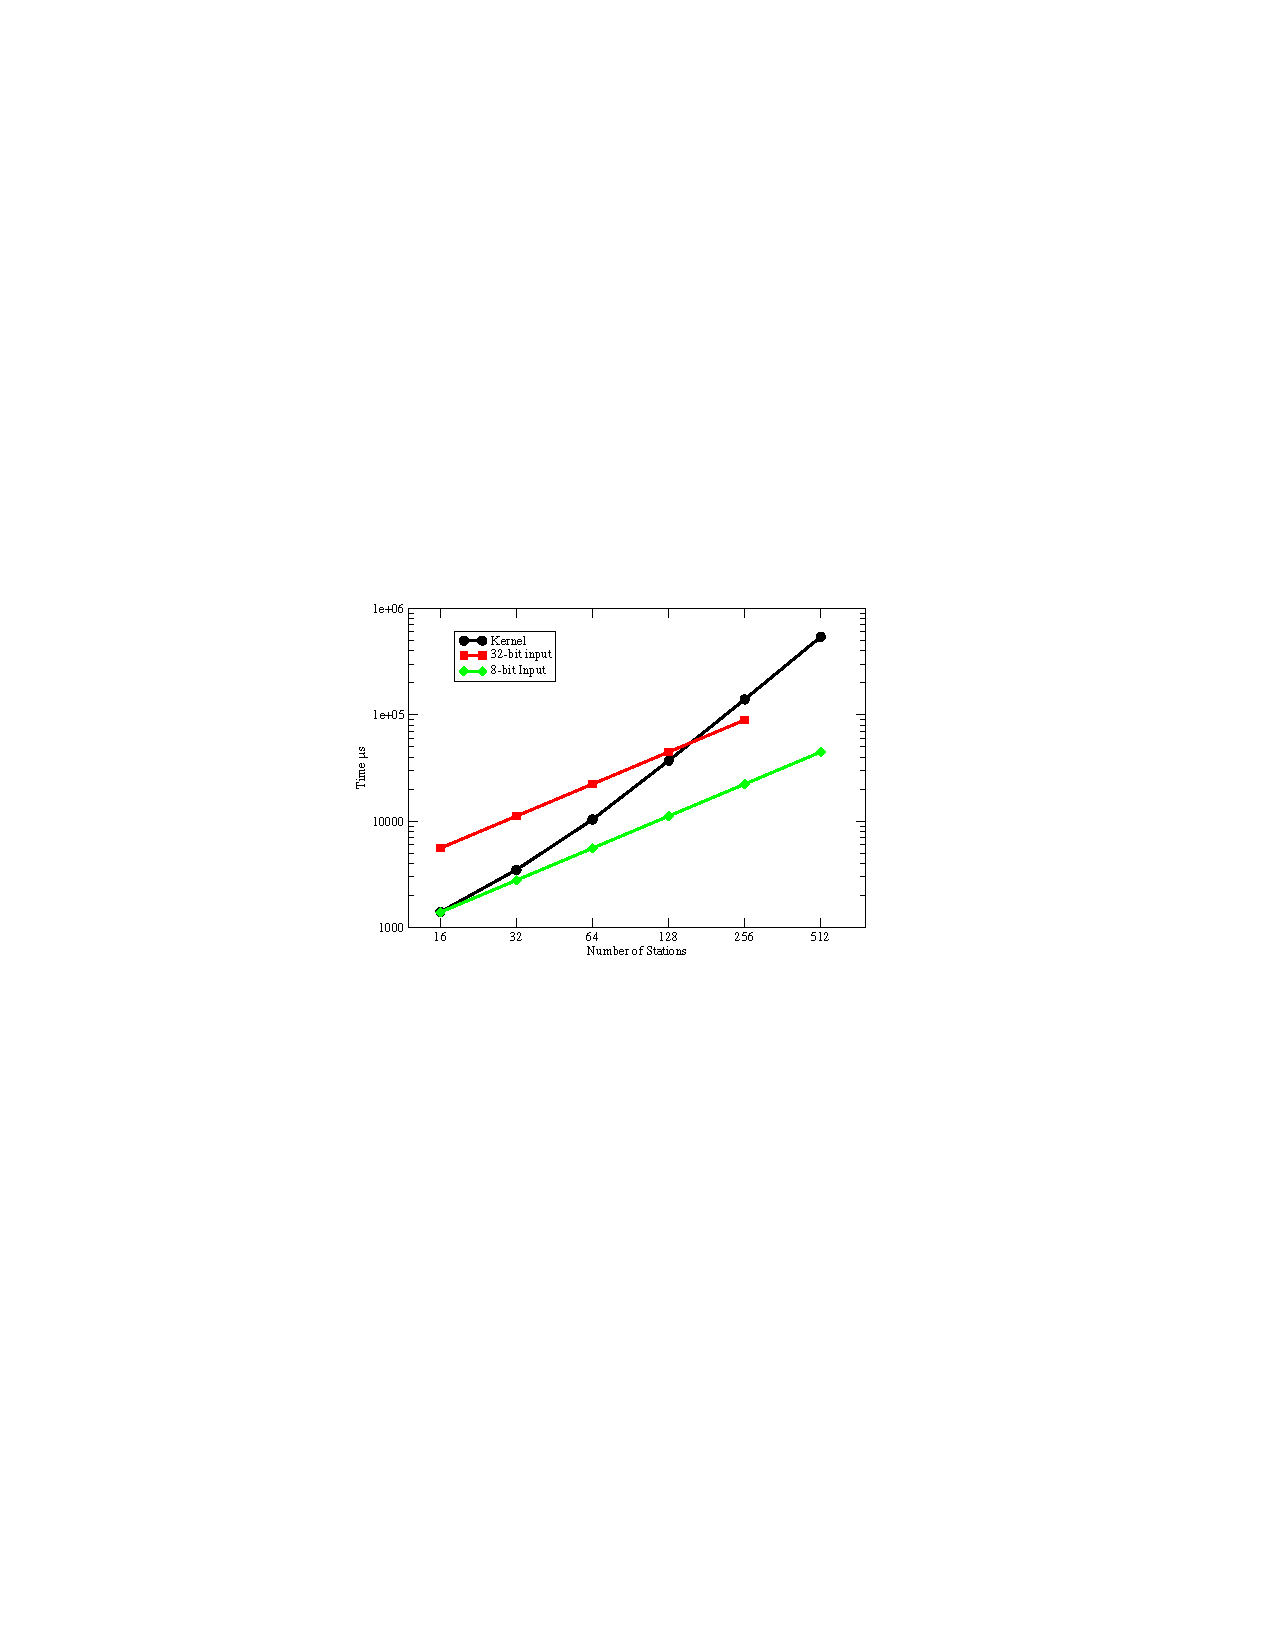
\includegraphics[width=\textwidth]{Images/C3/gpuxperformance.pdf}
  \caption[xGPU Performance]{xGPU Performance (reprinted from \citeauthor{Clark:2011wi} \cite{Clark:2011wi})}
  \label{fig: C3/gpuxperformance.pdf}
\end{figure}

\cite{Clark:2011wi}

\cite{2009PASP..121..857W}


\subsection{CASPER}

At the Collaboration for Astronomy Signal Processing and Electronics Research (CASPER), we are developing  common libraries and hardware that can be used by radio astronomers developing instrumentation. The mission statement, available on the group website casper.berkeley.edu, concisely summarizes the goals of the group:

\begin{quotation}
The primary goal of CASPER is to streamline and simplify the design flow of radio astronomy instrumentation by promoting design reuse through the development of platform-independent, open-source hardware and software.
Our aim is to couple the real-time streaming performance of application-specific hardware with the design simplicity of general-purpose software. By providing parameterized, platform-independent "gateware" libraries that run on reconfigurable, modular hardware building blocks, we abstract away low-level implementation details and allow astronomers to rapidly design and deploy new instruments.
\end{quotation}

The collaboration, started at UC Berkeley by Dan Werthimer, Don Backer, and Mel Wright, has spread to include astronomers all over the world, as shown in Figure \ref{fig: C3/casper_collaborators.png}. 
The group collaborates with many large digital engineering groups including groups from the Jet Propulsion Laboratory (JPL), the National Radio Astronomy Observatory (NRAO), the Arecibo Observatory, SKA South Africa, and the Giant Metrewave Radio Telescope (GMRT) in India. 
The diversity and far reach in this collaboration ensures that the tools continue to be general purpose and widely accessible. 


\begin{figure}[h!]
  \centering
    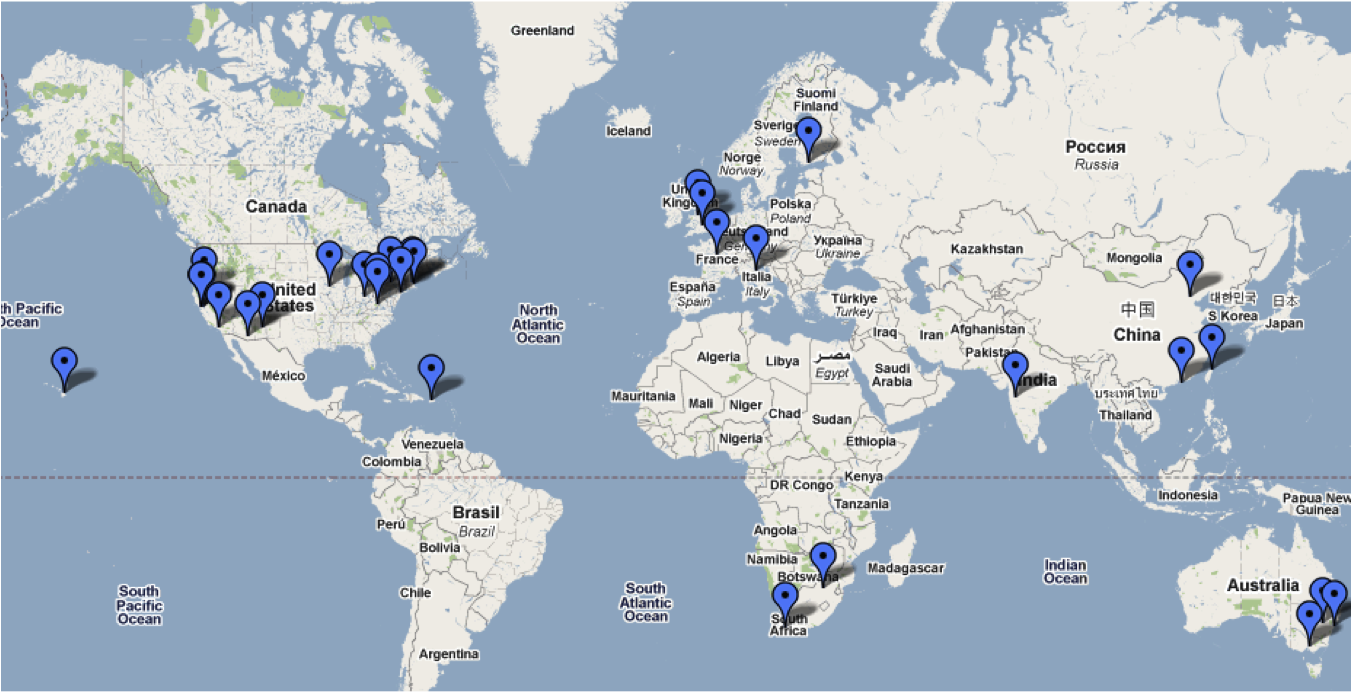
\includegraphics[width=\textwidth]{Images/C3/casper_collaborators.png}
  \caption{Map of CASPER Collaborators}
  \label{fig: C3/casper_collaborators.png}
\end{figure}

The CASPER FPGA libraries were developed to mitigate the need to redevelop common signal processing blocks for every new instrument \cite{Parsons:2006cu}. 
The library provides parameterized blocks such as FFTs, digital down-converters, and FIR filters that are the necessary building blocks for a wide range of instruments. 
Coupled with open source FPGA boards, such as the ROACH (Reconfigurable Open Architecture Computing Hardware), the CASPER libraries provide a useful toolbox for radio astronomy instrumentation development.
The follow sections describe each of these and how they have been used to create a number of different instruments.



\subsubsection{CASPER Hardware}

The CASPER group provides set of modular FPGA boards and ADCs that are designed specifically to deal with the high bandwidth requirements of real time radio astronomy signal processing. 
Since each FPGA boards meets the needs of the radio astronomy community as a whole rather than a single application, the group releases a small number of boards and typically only releases a new board to take advantage of improving technology. 
By releasing a handful of boards, the CASPER group ensures that users get proven and tested hardware for their new instruments.
The CASPER library and software, discussed below, also make it easy to upgrade the hardware since a CASPER design easily be recompiled to work with a different board and the software interface and the signal processing model are standardized.
And, since the boards communicate over a common set of industry standard protocols, they can be upgraded one by one, or all at once. 

Each FPGA board implements a number of high speed interfaces to send and receive data.
The Z-DOK+ connectors are primarily used to interface the boards to high speed ADCs and DACs.
This common Z-DOK+ interconnect implemented on nearly all CASPER ADC boards allows the astronomer to choose an ADC to match their scientific goals. 
The diversity of available boards is shown in Table \ref{tab: C3/adcs}.

\begin{table}
\centering
\begin{tabular}{| l | l | l | l |}
\hline  
\textbf{ADC Name} & Max sample rate & Streams & Bitwidth \\
\hline  
64ADCx64-12 & 50 Msps & 64 & 12 bits\\
ADC4x250-8 or QuadADC & 250 Msps & 4 & 8 bits\\
KatADC & 1.5 Gsps & 1 & 8 bits  \\
ADC1X2200-10 & 2.2 Gsps & 1 & 10 bits \\
ADC1x10000-4 & 10 Gsps & 1 & 4 bits \\
\hline  
\end{tabular}
\caption{CASPER ADC Boards}
\label{tab: C3/adcs}
\end{table} 




Each board can also send or receive data using ethernet. 
The boards are designed to communicate using common protocols, like 10 Gigabit Ethernet, so a board can be upgraded without modifying how it communicates with the rest of the cluster. 
The use of an industry standard protocol also makes communication to non-CASPER boards simple, allowing an FPGA to create UDP packets that eventually get received by a CPU or GPU-based server, making the CASPER boards an ideal component in a heterogeneous cluster. 
This makes it simple to design a cluster, and allows continuous upgrades as technology improves, as the signal processing model and communication model do not change between boards.


%Can�t clock FPGA at 3GHz but use parallel FFT 8-16 samples at a time
%BEE2 lib w/Bob Broderson

\begin{figure}[ht!]
  \centering
    \includegraphics[width=\textwidth]{Images/C3/roach.pdf}
  \caption{ROACH Board}
  \label{fig: C3/roach.pdf}
\end{figure}

Currently, CASPER has designed the IBOB, or Interconnect Break-out Board, ROACH and ROACH2 boards. 
The IBOB was originally designed as an interface to digitize antenna data and send it to a server, but the powerful Virtex-II Pro make it very useful for channelizing data as well.
The ROACH board is shown in Figure \ref{fig: C3/roach.pdf} with an iADC board connected via Z-DOK+ and an ethernet cable to get data off the board,
This board is pin-compatible with two large FPGA chips, the Virtex 5 SX95T and LX100T, with the SX95T being preferred for its large number of DSP-48s.
The ROACH has 2 Z-DOK+ connectors and supports up to 4 10-gigabit Ethernet links.
The ROACH2 is an upgrade to the ROACH board to take advantage of the newer Xilinx chips.
The Virtex 5 chips have been upgraded to the Virtex 6 SX475T, and this board supports up to 8 10-gigabit Ethernet links.



\subsubsection{CASPER Library}

In addition to hardware, CASPER develops a DSP library that can be compiled into an FPGA bitstream.
The library is implemented in Simulink, which allows for both simulation and, using Xilinx System Generator, compilation to FPGA code.
The Simulink implementation is a key part of the success of this project.
Using a visual programming language makes it easy to snap together blocks without getting into the low level details of FPGA programming.




%  Platform independent DSP library

%  Matlab scripts (�mask scripts�) are used to configure parameterized blocks

\begin{figure}[!h]
  \centering
    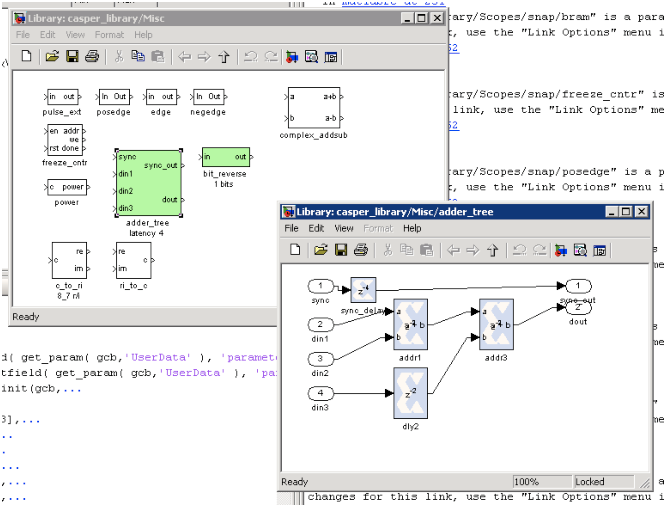
\includegraphics[width=\textwidth]{Images/C3/adder_tree_diagram.pdf}
  \caption{Adder Tree Simulink Simulink Diagram}
  \label{fig: C3/adder_tree_diagram}
\end{figure}



The library blocks are built out of Xilinx System Generator primitive blocks. 
These primitives make it possible to retarget Simulink designs to different Xilinx FPGAs without changed the original implementation.
Figure \ref{fig: C3/adder_tree_diagram} shows a simple example of one of the library blocks, an adder tree.
The adder tree is used to implement pipeplined, parallel addition using a binary tree.
The top left is the library with the adder tree block, and the bottom right is the implementation of the adder tree block with there inputs.

\begin{figure}[!h]
  \centering
    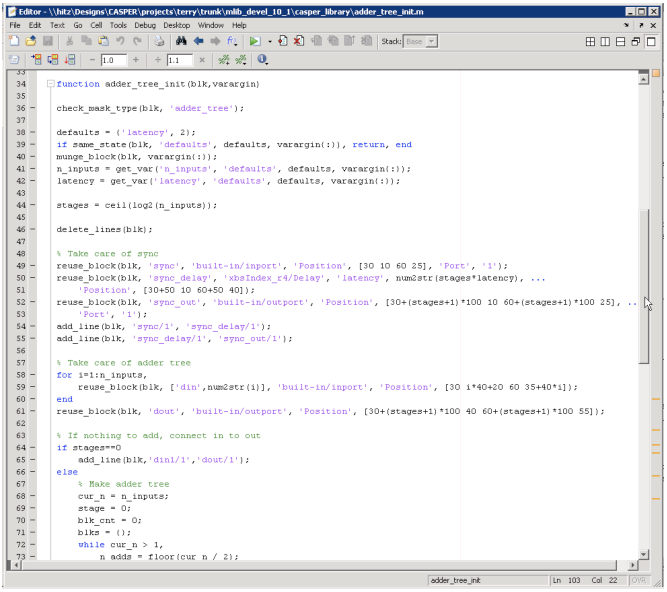
\includegraphics[width=\textwidth]{Images/C3/adder_tree_code.pdf}
  \caption{Adder Tree Simulink Mask Script}
  \label{fig: C3/adder_tree_code.pdf}
\end{figure}


In order to configure the number of inputs, Matlab scripts are used to redraw the implementations. 
Figure \ref{fig: C3/adder_tree_code.pdf} shows a snippet of code from the script used to redraw the adder tree block.
Every parameterized CASPER block uses at least one of these scripts to redraw the underlying implementation when the parameters are modified.
 

\begin{figure}
  \centering
     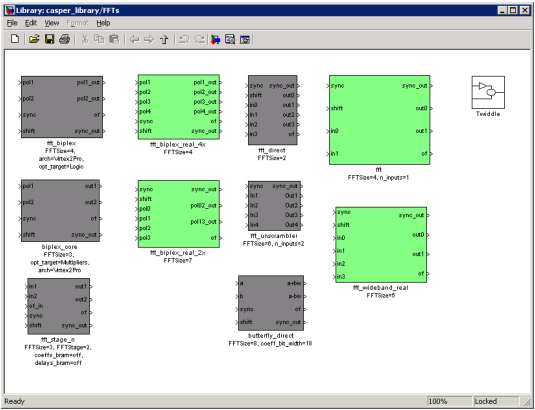
\includegraphics[width=\textwidth]{Images/C3/casper_fft_lib.pdf}
  \caption{CASPER FFT Library}
  \label{fig:casper_fft_lib.pdf}
\end{figure}

%TODO: remove this is achieved by
The CASPER library includes commonly used DSP blocks in radio astronomy instruments.
For example, the CASPER library provides FFTs, FIR filters, accumulators, digital downconverters, digital mixers which can be linked together to make an instrument. 
Each block is parameterized, making them useful for a variety of instruments. 
Figure \ref{fig:casper_fft_lib.pdf} shows the FFT library, which contains different types of FFTs, including blocks that can process multiple samples in parallel and blocks that are optimized to compute the FFT of a real signal. 


\begin{figure}
  \centering
     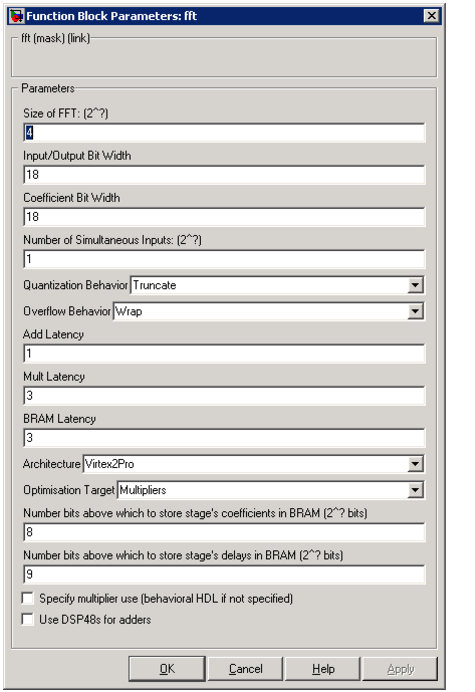
\includegraphics[width=0.45\textwidth]{Images/C3/casper_fft_lib_options.pdf}
  \caption{CASPER FFT Options Menu}
  \label{fig:casper_fft_lib_options.pdf}
\end{figure}


Figure \ref{fig:casper_fft_lib_options.pdf} shows the options menu for one of the FFT blocks. 
In order to support a variety of instruments, this block can be reconfigured to support different FFT lengths.
There are a number of other parameters provided like input bit width, which helps support a number of different ADCs or preprocessing algorithms, and FPGA-specific parameters like add latency, and multiply latency which have no effect on the result of the computation but change how the FFT gets mapped into hardware. 

\begin{figure}[ht!]
  \centering
    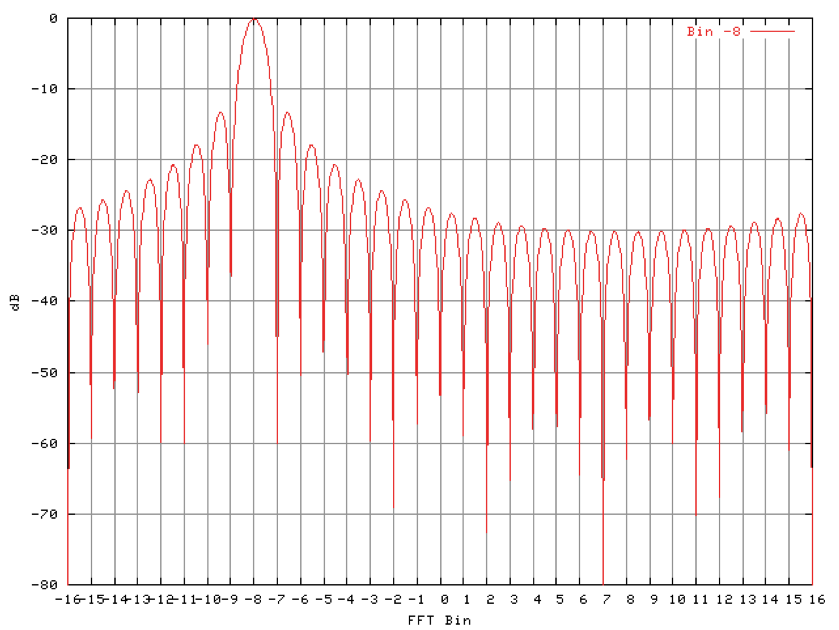
\includegraphics[width=0.48\textwidth]{Images/C4/fft_response.png}
    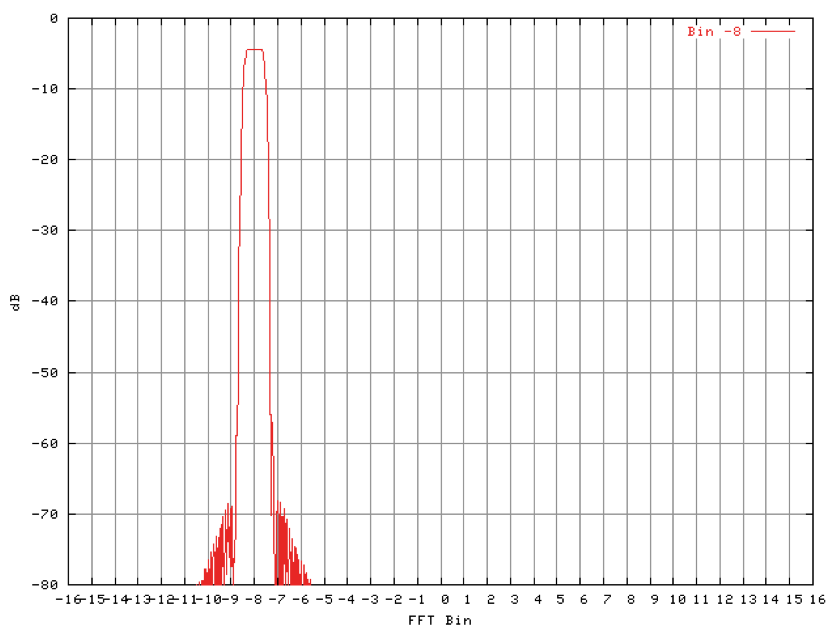
\includegraphics[width=0.48\textwidth]{Images/C4/pfb_response.png}
  \caption{A comparison of FFT and PFB response}
  \label{fig: fft_vs_pfb_response}
\end{figure}

The CASPER library also provides an FIR filter than can be coupled with the FFT to create a polyphase filter bank or PFB.
Figure \ref{fig: fft_vs_pfb_response} shows a comparison between the FFT and PFB response. 
The FFT response (on the left) has a lot of spectral leakage while the PFB (on the right) has a much sharper filter shape and a better frequency response. 
Despite the additional FPGA resources required by the FIR filter before the FFT, many instruments implement a PFB rather than an FFT because of the superior frequency response.


%TODO: maybe break this down into separate blocks
\begin{figure}
  \centering
     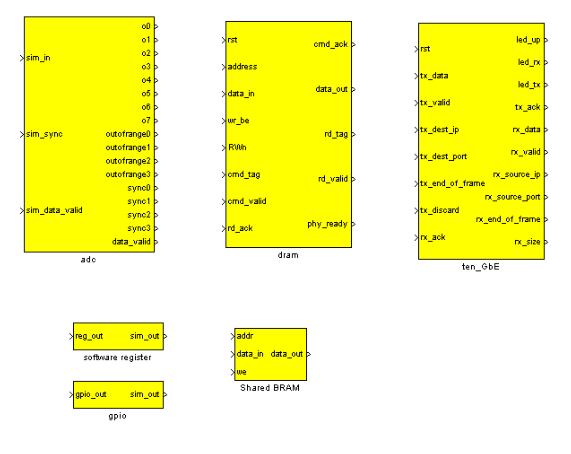
\includegraphics[width=0.75\textwidth]{Images/C3/yellow_blocks.pdf}
  \caption{CASPER Library IO Blocks}
  \label{fig:C3/yellow_blocks.pdf}
\end{figure}

The CASPER library also provides a set of blocks to abstract away the implementation of I/O interfaces, which are called yellow blocks. 
Figure \ref{fig:C3/yellow_blocks.pdf} provides some examples of what those library blocks look like. 
Each block provides input and output ports that correspond to the data it can send or receive. 
For example, the adc block has an output ports labeled \emph{o0,o1,\ldots,o7} that represent the data the FPGA receives from the iADC board.
In addition to this, simulation ports are provided to allow the user to proved test signals mimicking the outside world.
In the case of the ADC, the user could provide a sine wave into the \emph{sim\_in} port to observe how a sine wave would be processed by the system.
During compilation, the CASPER XPS toolflow automatically processes the blocks and ensures the wires are connected to the correct pins.


\subsubsection{CASPER Software}

To simplify the use of the FPGA further, the CASPER boards run a modified version of Linux directly on the board. 
Using this Linux environment, called the Berkeley Os for ReProgrammable Hardware or BORPH, programming the FPGA is as simple as running an executable on the command line \cite{So:2007ve}.
Once the board has been programmed, BORPH can communicate with the chip using an interface where some components on the FPGA like registers or memory appear as files in the operating system. 
These files can be accessed using normal file I/O, making it simple to send control signals or monitor the status of the chip, greatly simplifying debugging and command and control.


\subsubsection{SERENDIP V.v}

SERENDIP, or the Search for Extraterrestrial Radio Emissions from Nearby Developed Intelligent Populations, aims to find extra terrestrial intelligence by analyzing radio signals.
SERENDIP V.v is a high resolution SETI spectrometer that was deployed at Arecibo Observatory in 2009 as part of this project.
The installed instrument was built using an iADC, iBOB and BEE2 board.
THe instrument breaks up a single 200MHz stream into 128 million frequency channels, achieving a resolution of about 1Hz.

\begin{figure}[ht!]
  \centering
    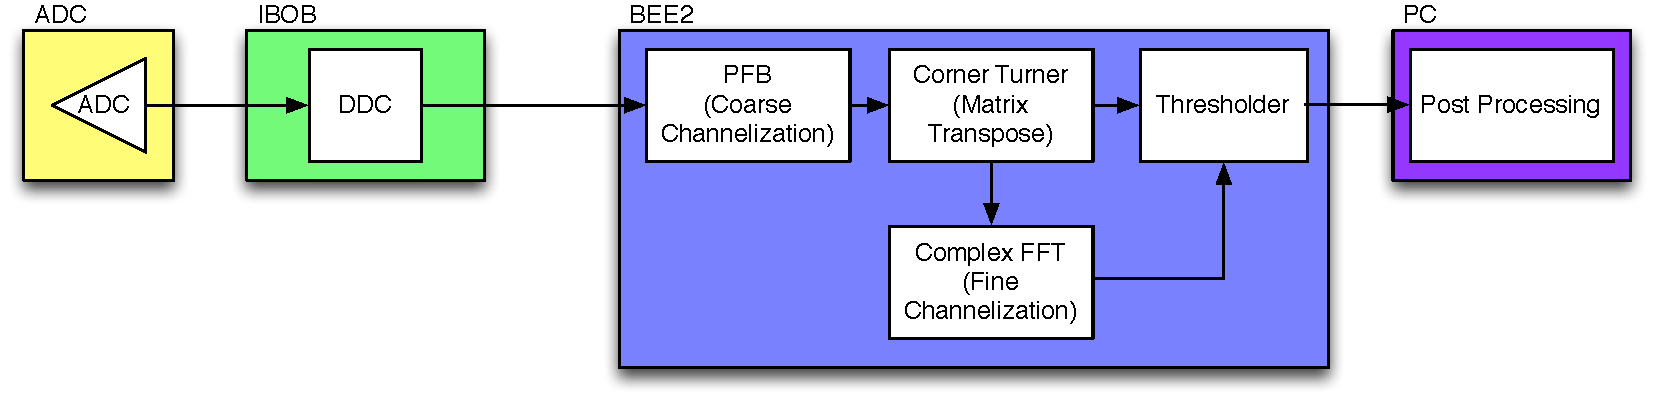
\includegraphics[width=\textwidth]{Images/C3/setispectrometerv55.pdf}
  \caption{SERENDIP V.v Block Diagram}
  \label{fig: C3/setispectrometerv55.pdf}
\end{figure}

Figure \ref{fig: C3/setispectrometerv55.pdf} shows the dataflow for the spectrometer.
The ADC data is fed into an IBOB where it is processed by a decimating downconverter. %TODO: why?


%4k point PFB
%  32k by 4k corner turn
%  32k point FFT
%  Each element (PFB, corner turn, FFT, and thresholder) is on a separate BEE2 chip
%  Output to PC is low bandwidth due to thresholding
%  Upcoming ROACH architecture will support 2 polarizations, 400 MHz


%Used for the SETI ALFA Survey, JPL Sky Survey, and Argentina SETI
%  200 MHz Bandwidth currently, future plans to upgrade to 300MHz
%  Build using an iADC, iBOB and BEE2
%  Can process one polarization from a single beam

\begin{figure}[ht!]
  \centering
    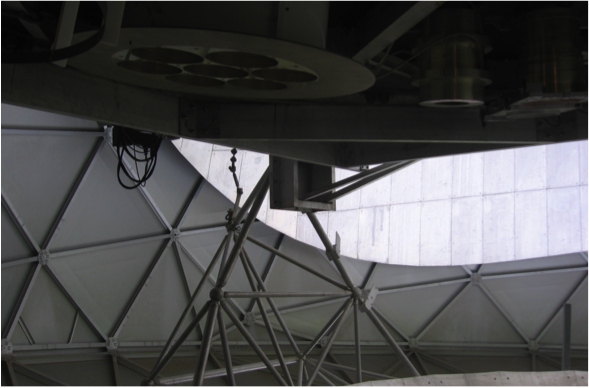
\includegraphics[width=\textwidth]{Images/C3/alfa_feed.png}
  \caption{Arecibo ALFA Feed}
  \label{fig: C3/alfa_feed.png}
\end{figure}

The SERENDIP V.v instrument processes data from the Arecibo L-band Feed Array.
The array has 7 dual-polarization beams, shown in Figure \ref{fig: C3/alfa_feed.png}.
The spectrometer


\begin{figure}[ht!]
  \centering
    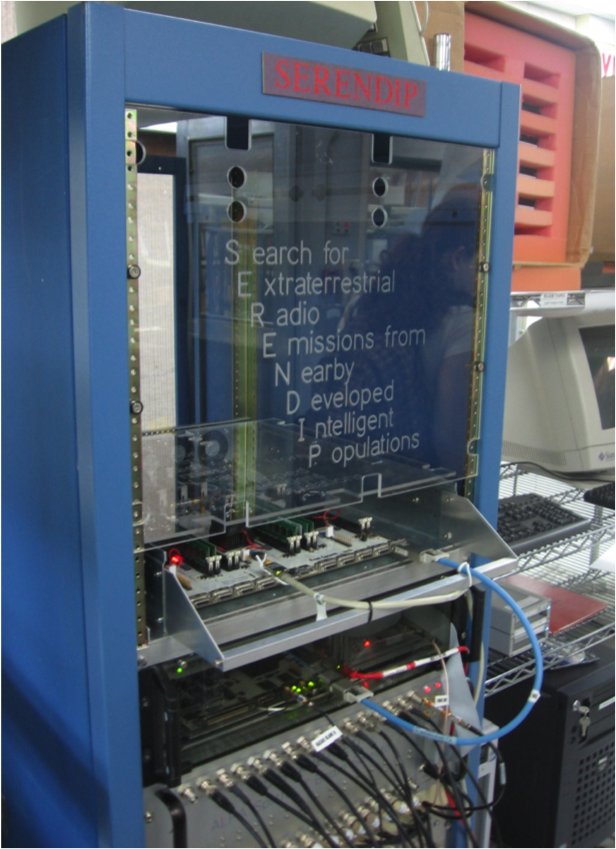
\includegraphics[width=0.48\textwidth]{Images/C3/serendip_vv_top.png}
    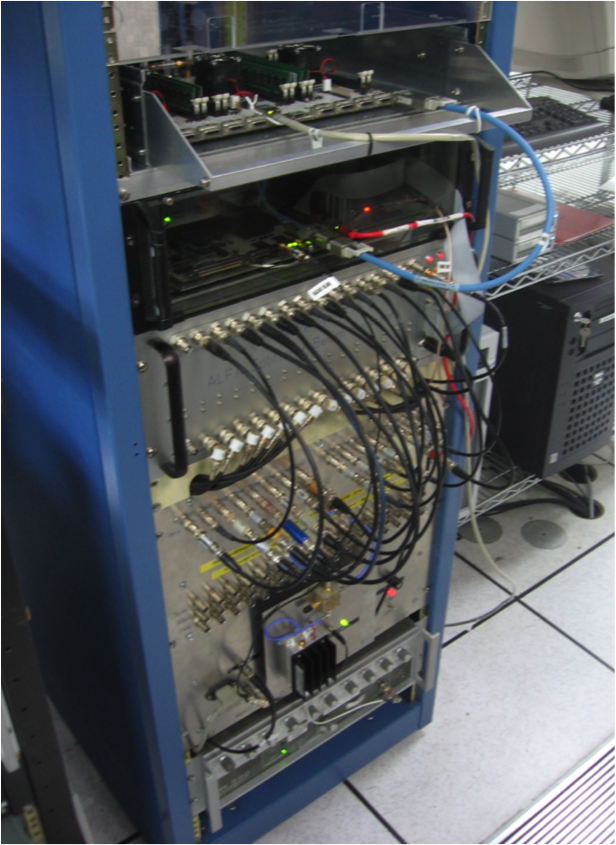
\includegraphics[width=0.48\textwidth]{Images/C3/serendip_vv_bottom.png}
  \caption{SERENDIP V.v Hardware installed at Arecibo Observatory}
  \label{fig: C3/serendipvv}
\end{figure}

Figure \ref{fig: C3/serendipvv} shows the installed instrument at Arecibo Observatory. 



%SuccessfullydeployedatAreciboObservatoryinJune2009
%  ImplementedonanIBOBandBEE2board
%  200MHzbandwidth
%  28million(227)channels(4kcoarsechannels*32kfinechannels)
%  1. 5 Hz/channel
%  0. 67 sec integration time
%  ObservescommensallywithallALFAobservations
%  Observesonlyonebeamatatime

%Arecibo L-band Feed Array
%?  7 pixel dual polarization ?  ALFA RF 1225-1525 MHz

\cite{2010LPICo1538.5378S}


\subsubsection{CASPER Correlator}
\begin{figure}[ht!]
  \centering
    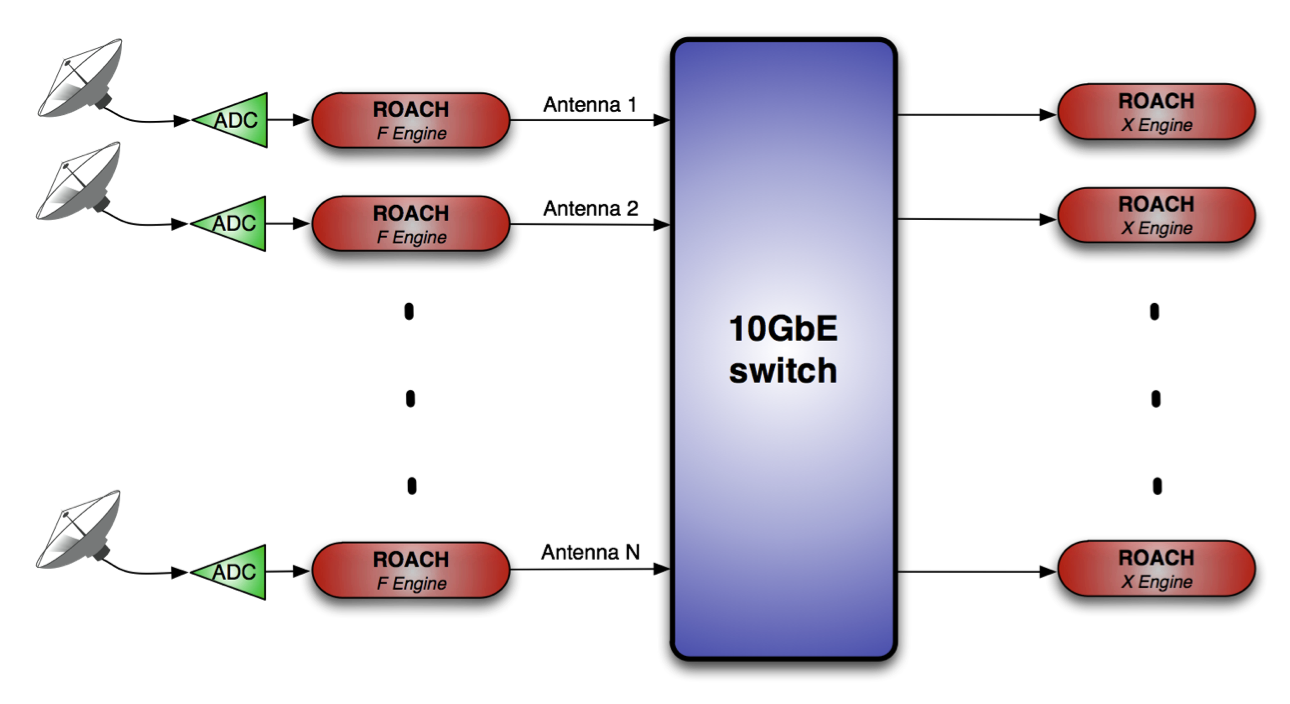
\includegraphics[width=\textwidth]{Images/C3/casper_correlator.png}
  \caption{CASPER Correlator Block Diagram}
  \label{fig: C3/casper_correlator.png}
\end{figure}

\cite{Parsons:2008dl}

%Used to develop Parsons/Manley correlator
%10GbE switch solves cabling problem
%Still have N^2 X engines

\subsection{Packetized Astronomy Signal Processor}

%TODO
%\cite{McMahon:2008tk}

Many radio astronomy instruments channelize the antenna data as soon as it is digitized. 
PASP implements a parameterized, FPGA-based channelizer, shown in Figure \ref{fig: pasp_fpga_arch}.
The FPGA interfaces to an ADC board that simultaneously digitizes 2 signals. 
The samples are sent into a polyphase filter bank (PFB), consisting of an FIR filter and an FFT, which breaks up the entire bandwidth sampled by the ADC into smaller subbands.
After dividing up the subbands, each band is rescaled. 
This step allows us to compensate for the shape of the analog filter feeding data into the ADC. 
After rescaling, the FPGA forms packets where each packet contains data from a single subband.
The packets are sent out over CX4 ports to a 10 gigabit Ethernet switch.

\begin{figure}[h!]
  \centering
    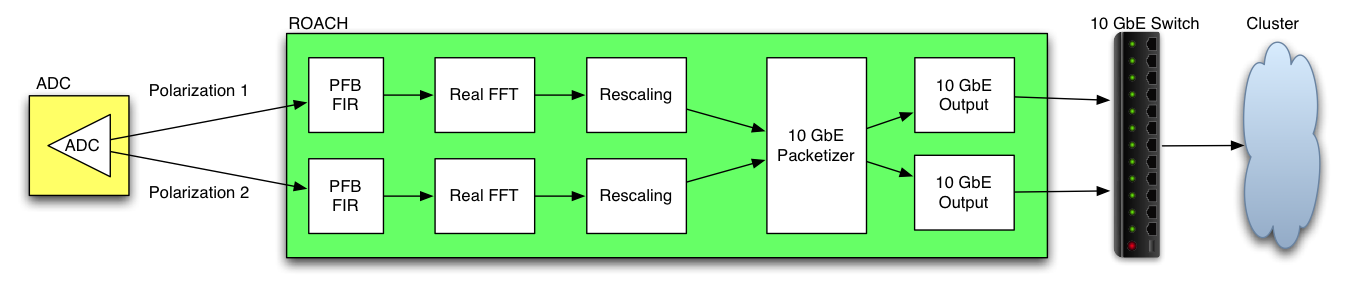
\includegraphics[width=1\textwidth]{Images/C4/pasp_fpga_arch.png}
  \caption{PASP Dataflow}
  \label{fig: pasp_fpga_arch}
\end{figure}



PASP is designed for flexibility. 
Building on the CASPER goal to automate the design of commonly used signal processing elements such as FFTs and digital downconverters, PASP automatically designs an entire FPGA instrument using only a few parameters.
The user can input the desired number of subbands, CPU/GPU cluster size, and packet size and a new design is automatically generated in Simulink.  
Figure \ref{fig: C4/pasp_high_level_interface.png}

\begin{figure}[h!]
  \centering
    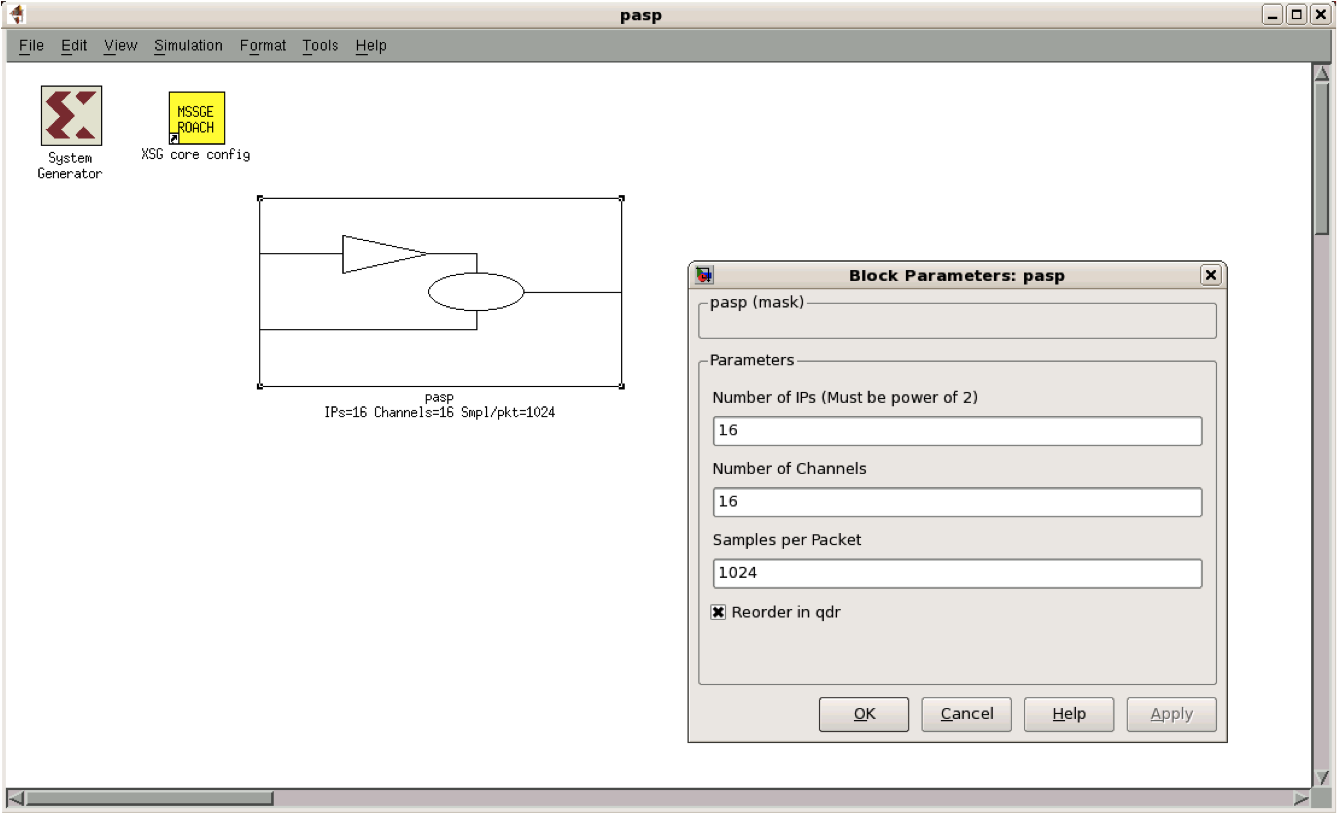
\includegraphics[width=1\textwidth]{Images/C4/pasp_high_level_interface.png}
  \caption{PASP Interface}
  \label{fig: C4/pasp_high_level_interface.png}
\end{figure}

The interface to PASP is a simple menu that consists of four parameters.
From the menu, \emph{Number of IPs} determines the number of IP addresses the instrument will need to send data to, defined by the size of the cluster it must communicate with.
\emph{Samples per Packet} defines the packet size, adjustable to ensure that the packet rate is low enough for the server to handle.
And \emph{Number of Channels} defines the FFT length.
The last parameter \emph{Reorder in QDR}, allows the packet buffering to be handled by off chip QDR memory.
This is only a parameter and not the default because it is only supported by certain boards.

\begin{figure}[h!]
  \centering
    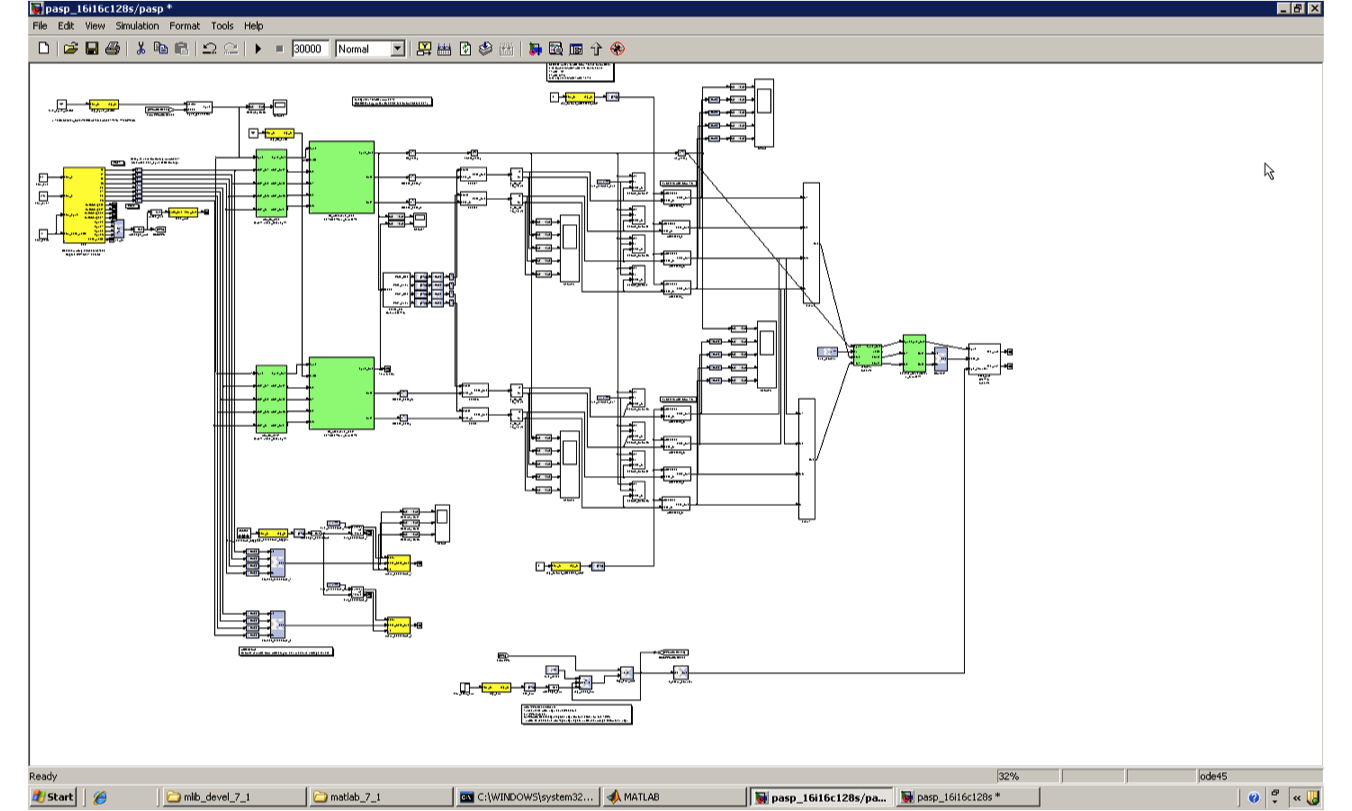
\includegraphics[width=1\textwidth]{Images/C4/pasp_low_level.png}
  \caption{PASP Low Level Implementation}
  \label{fig: C4/pasp_low_level.png}
\end{figure}

Changing any parameter causes the entire low-level design to be redrawn. 
Figure \ref{fig: C4/pasp_low_level.png} shows the low level implementation of the instrument.
Although this diagram is complex. it is generated automatically by PASP and the user never needs to look at this design to implement a working instrument.

PASP has a wide variety of potential applications due to the flexibility of the server software. 
In the next sections, we describe a few specific applications than can make use of this package.

\subsubsection{Pulsar Processing}
This design also has applications in pulsar science. 
The fast channelization on the FPGA with no data reduction makes it an ideal pulsar spectrometer, since no information is lost before sending the data to the servers.
GPUs provide a good platform for pulsar processing algorithms such as coherent dedispersion \cite{Ransom:2009wz}, which can easily be used as the processing function for the server software distributed in our package. 
Similar to SETI instruments, pulsar instruments designed using this package can also keep up with improvements in technology with a simple recompile.

%TODO: add info about deployed instruments
This design has been used in pulsar processors that have been deployed at the Parkes Observatory, Nan�ay Decimetric Radio Telescope, and Effelsberg Radio Telescope.

\subsubsection{Heterogeneous Radio SETI Spectrometer}

In the search for extraterrestrial intelligence (SETI), the ability to keep up with changes in technology allows searching instrumentation to stay on the leading edge of sensitivity. 
SETI aims to process the maximum bandwidth possible with very high resolution spectroscopy.
This instrument allows SETI projects to easily keep up with improvements on the telescope and increasing computational power.
An increase in detector bandwidth, improving the breadth of the search, can be processed simply recompiling the FPGA design and distributing the extra subbands to new servers. 
As computation improves, the instrument can be reconfigured to send more bandwidth to each computer, reducing the required cluster size, or improve the resolution of the instrument by doing a larger FFT on the server.

\begin{figure}[h!]
  \centering
    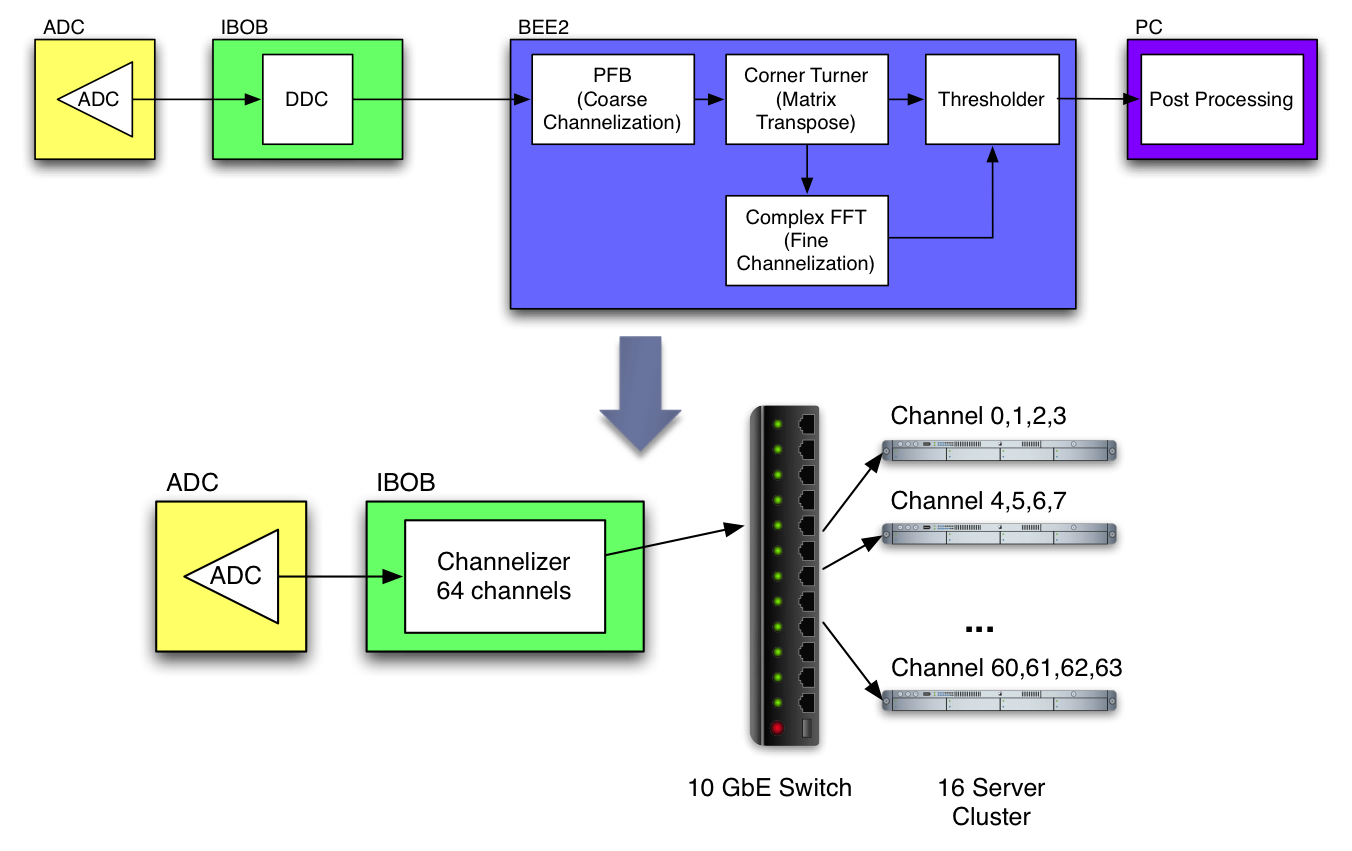
\includegraphics[width=\textwidth]{Images/C4/serendip_vv_to_hrss.png}
  \caption{TODO}
  \label{fig: C4/serendip_vv_to_hrss.png}
\end{figure}

The design of HRSS is based on the Serendip V.v design presented in Section \ref{Related Work:Radio Astronomy}.
Figure \ref{fig: C4/serendip_vv_to_hrss.png} shows how in HRSS the IBOB and BEE2 are replaced with a single chip FPGA board such as an IBOB or ROACH, and the fine channelization, thresholding and post processing are done on a GPU.

Unlike Serendip V.v, HRSS is a software package to automatically generate spectrometers with minimal user input.
We have automated the design of the spectrometer, creating a parameterized spectrometer that only requires a recompile to implement a change in specification.
This spectrometer combines FPGAs running PASP with GPUs, doing coarse channelization on the FPGA and sending each subband to the GPUs for further processing.
The server software is designed for flexibility, allowing astronomers to easily modify the processing algorithm run on the GPU and customize the instrument to fit their science goals.

The software package is comprised of two parts, the PASP design that runs on the FPGA and the server software.
Like PASP, the server software is parameterized, supporting a variety of spectral resolutions and integration times.
This software receives data over an Ethernet port and transfers it from the CPU to the GPU. 
The GPU runs an FFT and then sends the data back to the CPU to be recorded.
The GPU software, like the GPU benchmark, uses the CUFFT library to run FFT. 
This allows for rapid deployment of a working spectrometer that is configured to take full advantage of available computing resources.
%Our general purpose approach allows for the rapid development of new instruments.

Figure \ref{fig:spec_highlevel} shows a high level view of a spectrometer that could be designed with this package. 
In this example, a ROACH board divides the input band into 64 subbands and sends them out to a 16 server cluster.
An ADC is used to digitize data from the telescope and connects to the ROACH board via Z-DOK connectors. 
The digitized data is split into 64 subbands and sent through a 10 gigabit Ethernet switch.
Each server in the cluster receives and processes 4 subbands.

\begin{figure}[ht!]
  \centering
     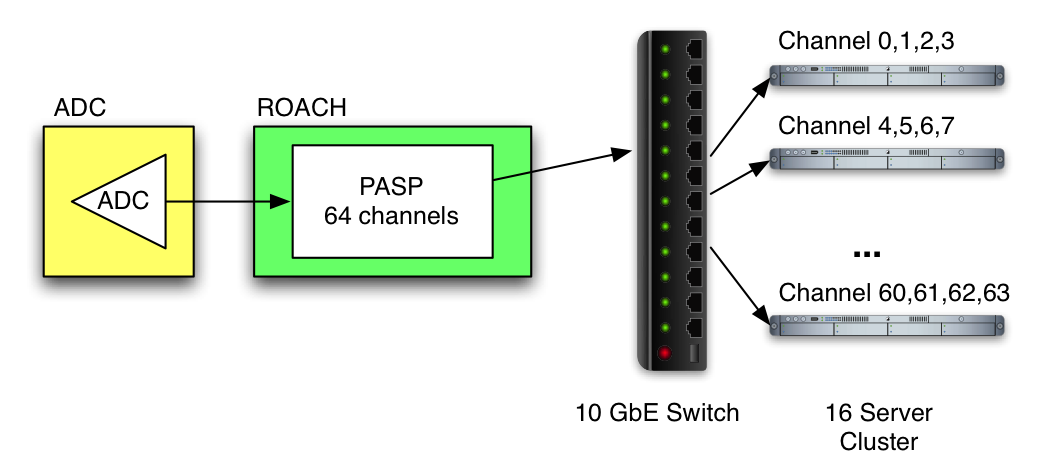
\includegraphics[width=1\textwidth]{Images/C4/spec_highlevel.png}
  \caption{Example high level spectrometer architecture}
  \label{fig:spec_highlevel}
\end{figure}

The server software was designed so other applications could easily be implemented on the GPU without altering or rewriting the receive code that interprets the packet headers and transfers data to the GPU.
Once the data is on the GPU, the software calls a process function and passes it a pointer to the GPU data.
An initialization function is called before the data processing begins to do any setup needed by the processing function, and an corresponding destroy function cleans up once the processing is complete.
In the spectroscopy software included in the package, the initialization function creates the FFT plan, the processing function calls CUFFT, and the destroy function deletes the FFT plan.
Modifying the application run on the GPU simply requires a redefinition of these three functions.
Using this interface, we successfully replaced the CUFFT processing with software developed for SETI searches designed by Kondo et al. \cite{Kondo:2010uk}.


\section{Tuning} \label{Related Work:Tuning}
\subsection{Metropolis}

The Metropolis project focused on mapping algorithms onto embedded systems \cite{Davare:2007ue}. 
The tool provides a framework for an abstract block based description of the algorithm. 
This description makes it easy to stitch algorithms together without specifying the eventual hardware implementation, providing a simple path to simulation and algorithm development that is separate from the implemented design. 
Then, the tool automatically maps the description onto an existing heterogeneous embedded system. 

%TODO: review references
\cite{Balarin:2003kc}
\cite{Densmore:tm}

%Mapping is focused on scheduling onto heterogeneous platforms
%Strong focus on embedded systems

%Some people have thought about how to use technology
%Metropolis works on simulation extensively (supporting 
%Embedded systems � we have 1 cpu and 1 dsp let�s make it go fast
%This doesn�t solve our problem
%Just does scheduling

The mapping generated by the tool is simply a schedule, specifying where and when each part of the computation gets executed. 
The tool seeks to optimize performance of the algorithm, ensuring the generated schedule runs as fast as possible on the hardware provided. 
This technique requires a fixed hardware model and uses the existing hardware to optimize performance. 
While this work is useful when a hardware model exists, it does not provide any flexibility in the hardware model while mapping the algorithm. 
So, when it is necessary to design the hardware to begin with, this does not solve the problem. 

%Doesn�t help design the cluster
%A �heterogeneous node� has a fixed mix of resources
%Can�t reduce costs by throwing away certain types of hardware
%Optimization is based on a fixed architecture and flexible performance
%Doesn�t match our �always running� model
%Performance is �good enough�, not an optimization target

Additionally, this type of solution is ill-suited to mapping the algorithms required to do real-time radio astronomy signal processing. 
This tool assumes it must schedule a discrete task onto a fixed piece of hardware and attempts maximize the performance of the task. 
In the applications described in Chapter \ref{chap:Real Time Radio Astronomy Algorithms}, the computation should always be running and needs to meet some minimum performance target.
Once the performance target is met, it is better to have a tool that will other costs like power or amount of hardware, rather attempting to improve the runtime of the algorithm. 








%Lisa Marie Guerra (?)


\subsection{Scheduling}
An integer linear programming model for mapping applications on hybrid systems

%TODO: sort these out
\cite{Gibeling:2008vg}

\cite{Theodoridis:2009gd}

\cite{Tsoi:2010we}

\cite{Jun:2008vv}

\cite{Rakhshanfar:2011tg}